\section{Human Hearing}

Sound is perceived differently from person to person. As a result, many products concerning sound is equipped with options to manipulate the sound produced in speaker system. But the main issue still lies in how the sound is perceived. In 1933 Harvey Fletcher and Wilden A. Munson conducted an experiment concerning the perception of sound based on subjective measurements from a diverse group of people. This experiment was later used to support the creation of IS0 226:2003 and the Fletcher-Munson equal-loudness contours, depicted on \autoref{fig:SoundPerceived}, which is accepted as the human perception of sound.

\begin{figure}[H]
\centering
\tikzsetnextfilename{FletcherMunson}
% This file was created by matlab2tikz.
%
%The latest updates can be retrieved from
%  http://www.mathworks.com/matlabcentral/fileexchange/22022-matlab2tikz-matlab2tikz
%where you can also make suggestions and rate matlab2tikz.
%
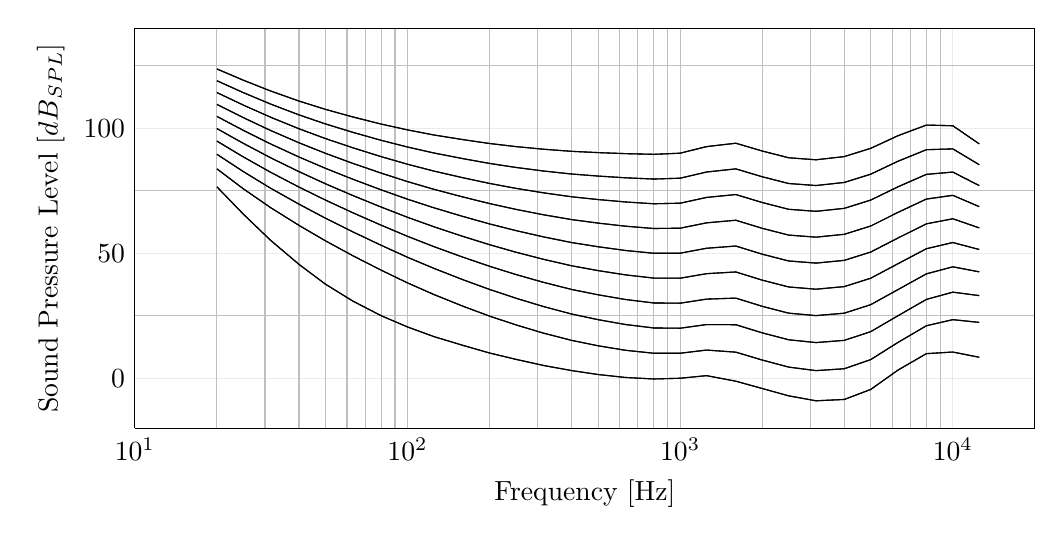
\begin{tikzpicture}

\begin{axis}[%
width=4.5in,
height=2in,
    grid = both,
    minor tick num=1,
    every major grid/.style={opacity=0.3},
    major tick length=0pt,
    minor tick length=0pt,
scale only axis,
separate axis lines,
every outer x axis line/.append style={black},
every x tick label/.append style={font=\color{black}},
xmode=log,
xmin=10,
xmax=20000,
xminorticks=true,
every outer y axis line/.append style={black},
every y tick label/.append style={font=\color{black}},
ymin=-20,
ymax=140,
ylabel={Sound Pressure Level [$\text{dB}_{\text{SPL}}$]},
xlabel={Frequency [Hz]},
axis background/.style={fill=white}
]
\addplot [color=black,solid,forget plot]
  table[row sep=crcr]{%
20	76.5517383226041\\
25	65.6188759741168\\
31.5	55.1228265549535\\
40	45.5339900534067\\
50	37.6321194195339\\
63	30.864980533887\\
80	25.0237914033185\\
100	20.5100135042932\\
125	16.6458196570746\\
160	13.116015107412\\
200	10.0882580994376\\
250	7.54356083431948\\
315	5.11374466782048\\
400	3.05885212574846\\
500	1.48243601230341\\
630	0.302918571977457\\
800	-0.302645737502345\\
1000	-0.0102578059037484\\
1250	1.03349848307708\\
1600	-1.186315801482\\
2000	-4.1115945810126\\
2500	-7.04616405279613\\
3150	-9.0260099416371\\
4000	-8.49438129744456\\
5000	-4.48287884775377\\
6300	3.2816607604897\\
8000	9.82911156789024\\
10000	10.4756869143707\\
12500	8.38134268048196\\
};
\addplot [color=black,solid,forget plot]
  table[row sep=crcr]{%
20	83.750025182093\\
25	75.7579476174299\\
31.5	68.2089105982577\\
40	61.1364793677951\\
50	54.9637937682932\\
63	49.0098436715886\\
80	43.2376895603486\\
100	38.1337745810234\\
125	33.4772204553404\\
160	28.7734160607378\\
200	24.8416951510023\\
250	21.3272275714054\\
315	18.0522420213635\\
400	15.1378821058428\\
500	12.9768236730699\\
630	11.179146489796\\
800	9.99175401339798\\
1000	9.9996188235628\\
1250	11.2621464205195\\
1600	10.4291304547924\\
2000	7.27444422402539\\
2500	4.45077959361514\\
3150	3.04041674970355\\
4000	3.79605666622204\\
5000	7.45829546247268\\
6300	14.3482692900305\\
8000	20.9841333243976\\
10000	23.4306375311977\\
12500	22.3269179096727\\
};
\addplot [color=black,solid,forget plot]
  table[row sep=crcr]{%
20	89.57808305545\\
25	82.6513213354879\\
31.5	75.9764274162507\\
40	69.6171278409198\\
50	64.0178112281964\\
63	58.5520257569407\\
80	53.1897958643328\\
100	48.3808999382271\\
125	43.9414107049108\\
160	39.3702034647556\\
200	35.5125839314343\\
250	31.9922270822934\\
315	28.6866338147182\\
400	25.6703001183791\\
500	23.4262503493827\\
630	21.4824972982365\\
800	20.1011194530384\\
1000	20.0051703947423\\
1250	21.4617803626109\\
1600	21.4012793902399\\
2000	18.1515477844233\\
2500	15.3843668219524\\
3150	14.2558997206244\\
4000	15.1414556800994\\
5000	18.6348681075747\\
6300	25.0195625279572\\
8000	31.5227463312565\\
10000	34.4255563813946\\
12500	33.0444150871593\\
};
\addplot [color=black,solid,forget plot]
  table[row sep=crcr]{%
20	94.8496368966944\\
25	88.5219041380507\\
31.5	82.3587077005053\\
40	76.4545124065439\\
50	71.2624052592352\\
63	66.1966316617882\\
80	61.2218987795272\\
100	56.76087709962\\
125	52.6368471259455\\
160	48.3825791604872\\
200	44.7777394712575\\
250	41.4726841525456\\
315	38.3640241188394\\
400	35.5004901046235\\
500	33.3698992047686\\
630	31.4902012528631\\
800	30.1094066208767\\
1000	30.008291493461\\
1250	31.6451727170551\\
1600	32.042927801905\\
2000	28.7625200865421\\
2500	26.0254491177356\\
3150	25.0450982503263\\
4000	26.0184699587117\\
5000	29.4242302636228\\
6300	35.4810661339093\\
8000	41.7446076653441\\
10000	44.5662466148994\\
12500	42.547919719576\\
};
\addplot [color=black,solid,forget plot]
  table[row sep=crcr]{%
20	99.8539233392895\\
25	93.944411435575\\
31.5	88.1659025311256\\
40	82.628676094348\\
50	77.7848709364585\\
63	73.0825453201854\\
80	68.4778868156873\\
100	64.3711493949554\\
125	60.5855032509532\\
160	56.7022467742482\\
200	53.408739777839\\
250	50.3992413958554\\
315	47.5774865960839\\
400	44.9766225935126\\
500	43.0506793674477\\
630	41.3391949955489\\
800	40.0617608259665\\
1000	40.0100463699522\\
1250	41.8194550821733\\
1600	42.5075687643746\\
2000	39.2296390995457\\
2500	36.5090098594403\\
3150	35.6089191370347\\
4000	36.649177086339\\
5000	40.007741134917\\
6300	45.8282813177135\\
8000	51.7968069331766\\
10000	54.2841302509476\\
12500	51.485907193908\\
};
\addplot [color=black,solid,forget plot]
  table[row sep=crcr]{%
20	104.719829018815\\
25	99.1446295914627\\
31.5	93.694366473176\\
40	88.4851406791841\\
50	83.9629983927261\\
63	79.6064179991378\\
80	75.3618603618885\\
100	71.6094668546422\\
125	68.169609998711\\
160	64.6785735608863\\
200	61.7209504720936\\
250	59.042661259521\\
315	56.5496466564374\\
400	54.2649516351239\\
500	52.5898246932425\\
630	51.1011927088892\\
800	49.9829429635048\\
1000	50.011033131655\\
1250	51.9886218771043\\
1600	52.8753058719074\\
2000	49.6176114796166\\
2500	46.9060784077049\\
3150	46.0502046071593\\
4000	47.1463512049238\\
5000	50.4790034572604\\
6300	56.1123480434011\\
8000	61.7561182795062\\
10000	63.779824548619\\
12500	60.1353379120974\\
};
\addplot [color=black,solid,forget plot]
  table[row sep=crcr]{%
20	109.511322266919\\
25	104.227897844122\\
31.5	99.0778682592629\\
40	94.1773186176094\\
50	89.963457309807\\
63	85.9434213095042\\
80	82.0534007221553\\
100	78.6546186273787\\
125	75.5634531409223\\
160	72.4743448009634\\
200	69.8643192892605\\
250	67.53483531585\\
315	65.391739829195\\
400	63.4509962661032\\
500	62.051179195912\\
630	60.8149594207501\\
800	59.8866837493279\\
1000	60.0115880039174\\
1250	62.1549142967122\\
1600	63.1893560447056\\
2000	59.961614531787\\
2500	57.2551501924531\\
3150	56.4238586323755\\
4000	57.5699383810385\\
5000	60.8882124959286\\
6300	66.3612505616992\\
8000	71.6639659846509\\
10000	73.1551040106779\\
12500	68.6307704505211\\
};
\addplot [color=black,solid,forget plot]
  table[row sep=crcr]{%
20	114.261989379846\\
25	109.247746837385\\
31.5	104.383236437501\\
40	99.7812111627055\\
50	95.868549432028\\
63	92.1801004935835\\
80	88.6415135243374\\
100	85.5957343784509\\
125	82.8545558983978\\
160	80.17222829725\\
200	77.9158045592802\\
250	75.9443248897055\\
315	74.1623802305921\\
400	72.5805330712618\\
500	71.4693589120705\\
630	70.5018183982902\\
800	69.780644195049\\
1000	70.0119000237355\\
1250	72.3195910695875\\
1600	73.473466109527\\
2000	70.2810594418385\\
2500	67.5774309413929\\
3150	66.7598748049935\\
4000	67.9526085327365\\
5000	71.262857328828\\
6300	76.5904871357067\\
8000	81.5431129645672\\
10000	82.4640385160455\\
12500	77.0420555813957\\
};
\addplot [color=black,solid,forget plot]
  table[row sep=crcr]{%
20	118.990010884022\\
25	114.23264214656\\
31.5	109.645682769609\\
40	105.336683261343\\
50	101.721369747086\\
63	98.3617851890704\\
80	95.1728961911629\\
100	92.4797225204951\\
125	90.0891628630488\\
160	87.8161677329853\\
200	85.9165502664082\\
250	84.3080405919044\\
315	82.8933588080547\\
400	81.6786059642434\\
500	80.8634370844215\\
630	80.1736132306195\\
800	79.669113465515\\
1000	80.0120754829116\\
1250	82.4833595292968\\
1600	83.7408179497261\\
2000	80.5867468595003\\
2500	77.8847085052807\\
3150	77.0748486939853\\
4000	78.3124140407\\
5000	81.618168704315\\
6300	86.8086987661392\\
8000	91.4061952762329\\
10000	91.7360867537153\\
12500	85.4067696355526\\
};
\addplot [color=black,solid,forget plot]
  table[row sep=crcr]{%
20	123.705395027303\\
25	119.198100457884\\
31.5	114.884304508559\\
40	110.865302503646\\
50	107.545211218569\\
63	104.512979943985\\
80	101.672816142939\\
100	99.3320080493807\\
125	97.2923934744959\\
160	95.430112181467\\
200	93.8890507103411\\
250	92.6462400228125\\
315	91.602195422737\\
400	90.7590831078866\\
500	90.2440175635456\\
630	89.8369580012748\\
800	89.5544975714848\\
1000	90.0121741500787\\
1250	92.6466172802421\\
1600	93.9987705774216\\
2000	90.8847144154127\\
2500	88.1835688280923\\
3150	87.3780282660524\\
4000	88.6594072150229\\
5000	91.9626405687338\\
6300	97.020721335463\\
8000	101.260267322155\\
10000	100.987523983214\\
12500	93.7455269359469\\
};
\addplot [color=black,solid,forget plot]
  table[row sep=crcr]{%
20	76.5517383226041\\
25	65.6188759741168\\
31.5	55.1228265549535\\
40	45.5339900534067\\
50	37.6321194195339\\
63	30.864980533887\\
80	25.0237914033185\\
100	20.5100135042932\\
125	16.6458196570746\\
160	13.116015107412\\
200	10.0882580994376\\
250	7.54356083431948\\
315	5.11374466782048\\
400	3.05885212574846\\
500	1.48243601230341\\
630	0.302918571977457\\
800	-0.302645737502345\\
1000	-0.0102578059037484\\
1250	1.03349848307708\\
1600	-1.186315801482\\
2000	-4.1115945810126\\
2500	-7.04616405279613\\
3150	-9.0260099416371\\
4000	-8.49438129744456\\
5000	-4.48287884775377\\
6300	3.2816607604897\\
8000	9.82911156789024\\
10000	10.4756869143707\\
12500	8.38134268048196\\
};
\addplot [color=black,solid,forget plot]
  table[row sep=crcr]{%
20	83.750025182093\\
25	75.7579476174299\\
31.5	68.2089105982577\\
40	61.1364793677951\\
50	54.9637937682932\\
63	49.0098436715886\\
80	43.2376895603486\\
100	38.1337745810234\\
125	33.4772204553404\\
160	28.7734160607378\\
200	24.8416951510023\\
250	21.3272275714054\\
315	18.0522420213635\\
400	15.1378821058428\\
500	12.9768236730699\\
630	11.179146489796\\
800	9.99175401339798\\
1000	9.9996188235628\\
1250	11.2621464205195\\
1600	10.4291304547924\\
2000	7.27444422402539\\
2500	4.45077959361514\\
3150	3.04041674970355\\
4000	3.79605666622204\\
5000	7.45829546247268\\
6300	14.3482692900305\\
8000	20.9841333243976\\
10000	23.4306375311977\\
12500	22.3269179096727\\
};
\addplot [color=black,solid,forget plot]
  table[row sep=crcr]{%
20	89.57808305545\\
25	82.6513213354879\\
31.5	75.9764274162507\\
40	69.6171278409198\\
50	64.0178112281964\\
63	58.5520257569407\\
80	53.1897958643328\\
100	48.3808999382271\\
125	43.9414107049108\\
160	39.3702034647556\\
200	35.5125839314343\\
250	31.9922270822934\\
315	28.6866338147182\\
400	25.6703001183791\\
500	23.4262503493827\\
630	21.4824972982365\\
800	20.1011194530384\\
1000	20.0051703947423\\
1250	21.4617803626109\\
1600	21.4012793902399\\
2000	18.1515477844233\\
2500	15.3843668219524\\
3150	14.2558997206244\\
4000	15.1414556800994\\
5000	18.6348681075747\\
6300	25.0195625279572\\
8000	31.5227463312565\\
10000	34.4255563813946\\
12500	33.0444150871593\\
};
\addplot [color=black,solid,forget plot]
  table[row sep=crcr]{%
20	94.8496368966944\\
25	88.5219041380507\\
31.5	82.3587077005053\\
40	76.4545124065439\\
50	71.2624052592352\\
63	66.1966316617882\\
80	61.2218987795272\\
100	56.76087709962\\
125	52.6368471259455\\
160	48.3825791604872\\
200	44.7777394712575\\
250	41.4726841525456\\
315	38.3640241188394\\
400	35.5004901046235\\
500	33.3698992047686\\
630	31.4902012528631\\
800	30.1094066208767\\
1000	30.008291493461\\
1250	31.6451727170551\\
1600	32.042927801905\\
2000	28.7625200865421\\
2500	26.0254491177356\\
3150	25.0450982503263\\
4000	26.0184699587117\\
5000	29.4242302636228\\
6300	35.4810661339093\\
8000	41.7446076653441\\
10000	44.5662466148994\\
12500	42.547919719576\\
};
\addplot [color=black,solid,forget plot]
  table[row sep=crcr]{%
20	99.8539233392895\\
25	93.944411435575\\
31.5	88.1659025311256\\
40	82.628676094348\\
50	77.7848709364585\\
63	73.0825453201854\\
80	68.4778868156873\\
100	64.3711493949554\\
125	60.5855032509532\\
160	56.7022467742482\\
200	53.408739777839\\
250	50.3992413958554\\
315	47.5774865960839\\
400	44.9766225935126\\
500	43.0506793674477\\
630	41.3391949955489\\
800	40.0617608259665\\
1000	40.0100463699522\\
1250	41.8194550821733\\
1600	42.5075687643746\\
2000	39.2296390995457\\
2500	36.5090098594403\\
3150	35.6089191370347\\
4000	36.649177086339\\
5000	40.007741134917\\
6300	45.8282813177135\\
8000	51.7968069331766\\
10000	54.2841302509476\\
12500	51.485907193908\\
};
\addplot [color=black,solid,forget plot]
  table[row sep=crcr]{%
20	104.719829018815\\
25	99.1446295914627\\
31.5	93.694366473176\\
40	88.4851406791841\\
50	83.9629983927261\\
63	79.6064179991378\\
80	75.3618603618885\\
100	71.6094668546422\\
125	68.169609998711\\
160	64.6785735608863\\
200	61.7209504720936\\
250	59.042661259521\\
315	56.5496466564374\\
400	54.2649516351239\\
500	52.5898246932425\\
630	51.1011927088892\\
800	49.9829429635048\\
1000	50.011033131655\\
1250	51.9886218771043\\
1600	52.8753058719074\\
2000	49.6176114796166\\
2500	46.9060784077049\\
3150	46.0502046071593\\
4000	47.1463512049238\\
5000	50.4790034572604\\
6300	56.1123480434011\\
8000	61.7561182795062\\
10000	63.779824548619\\
12500	60.1353379120974\\
};
\addplot [color=black,solid,forget plot]
  table[row sep=crcr]{%
20	109.511322266919\\
25	104.227897844122\\
31.5	99.0778682592629\\
40	94.1773186176094\\
50	89.963457309807\\
63	85.9434213095042\\
80	82.0534007221553\\
100	78.6546186273787\\
125	75.5634531409223\\
160	72.4743448009634\\
200	69.8643192892605\\
250	67.53483531585\\
315	65.391739829195\\
400	63.4509962661032\\
500	62.051179195912\\
630	60.8149594207501\\
800	59.8866837493279\\
1000	60.0115880039174\\
1250	62.1549142967122\\
1600	63.1893560447056\\
2000	59.961614531787\\
2500	57.2551501924531\\
3150	56.4238586323755\\
4000	57.5699383810385\\
5000	60.8882124959286\\
6300	66.3612505616992\\
8000	71.6639659846509\\
10000	73.1551040106779\\
12500	68.6307704505211\\
};
\addplot [color=black,solid,forget plot]
  table[row sep=crcr]{%
20	114.261989379846\\
25	109.247746837385\\
31.5	104.383236437501\\
40	99.7812111627055\\
50	95.868549432028\\
63	92.1801004935835\\
80	88.6415135243374\\
100	85.5957343784509\\
125	82.8545558983978\\
160	80.17222829725\\
200	77.9158045592802\\
250	75.9443248897055\\
315	74.1623802305921\\
400	72.5805330712618\\
500	71.4693589120705\\
630	70.5018183982902\\
800	69.780644195049\\
1000	70.0119000237355\\
1250	72.3195910695875\\
1600	73.473466109527\\
2000	70.2810594418385\\
2500	67.5774309413929\\
3150	66.7598748049935\\
4000	67.9526085327365\\
5000	71.262857328828\\
6300	76.5904871357067\\
8000	81.5431129645672\\
10000	82.4640385160455\\
12500	77.0420555813957\\
};
\addplot [color=black,solid,forget plot]
  table[row sep=crcr]{%
20	118.990010884022\\
25	114.23264214656\\
31.5	109.645682769609\\
40	105.336683261343\\
50	101.721369747086\\
63	98.3617851890704\\
80	95.1728961911629\\
100	92.4797225204951\\
125	90.0891628630488\\
160	87.8161677329853\\
200	85.9165502664082\\
250	84.3080405919044\\
315	82.8933588080547\\
400	81.6786059642434\\
500	80.8634370844215\\
630	80.1736132306195\\
800	79.669113465515\\
1000	80.0120754829116\\
1250	82.4833595292968\\
1600	83.7408179497261\\
2000	80.5867468595003\\
2500	77.8847085052807\\
3150	77.0748486939853\\
4000	78.3124140407\\
5000	81.618168704315\\
6300	86.8086987661392\\
8000	91.4061952762329\\
10000	91.7360867537153\\
12500	85.4067696355526\\
};
\addplot [color=black,solid,forget plot]
  table[row sep=crcr]{%
20	123.705395027303\\
25	119.198100457884\\
31.5	114.884304508559\\
40	110.865302503646\\
50	107.545211218569\\
63	104.512979943985\\
80	101.672816142939\\
100	99.3320080493807\\
125	97.2923934744959\\
160	95.430112181467\\
200	93.8890507103411\\
250	92.6462400228125\\
315	91.602195422737\\
400	90.7590831078866\\
500	90.2440175635456\\
630	89.8369580012748\\
800	89.5544975714848\\
1000	90.0121741500787\\
1250	92.6466172802421\\
1600	93.9987705774216\\
2000	90.8847144154127\\
2500	88.1835688280923\\
3150	87.3780282660524\\
4000	88.6594072150229\\
5000	91.9626405687338\\
6300	97.020721335463\\
8000	101.260267322155\\
10000	100.987523983214\\
12500	93.7455269359469\\
};
\end{axis}
\end{tikzpicture}%
\caption{Equal-loudness contours curves from ISO 226:2003, showing how sound is perceived. The curves shows the perception at specific SPL(phon) at 1Khz. The range of the curves span between 0 - 90 dB SPL with an 10 dB interval \citepalias{ISO226}.}
\label{fig:SoundPerceived}
\end{figure}
\autoref{fig:SoundPerceived} shows how sound in general is perceived. The curve gives the designer of a speaker a guideline for what to aim for in frequency response. From the curves, the following perceptions can be deducted:
\begin{itemize}
\item Lower frequency, $ < 700$ Hz, sounds are attenuated.
\item Midrange frequency, $700 \text{ Hz} < $ and $ > 5.5$ kHz, sounds are enhanced/amplified.
\item High frequency, $ 5.5 \text{ kHz} < $, sounds are attenuated.
\end{itemize}

A further investigation shows that frequency spectrum needed for speech lies in 300 Hz to 3.4 Khz \citep{sou:VoiceFundamentals}. From the evolutionary perspective it makes sense that human hearing is optimized for hearing other humans talk. The main conclusion from ISO 223:2003 is that people will have a tendency to wanting more gain in lower frequency sound. This problem can be resolved by equalization.


